\section{Discussion}

\begin{figure}
\centering 
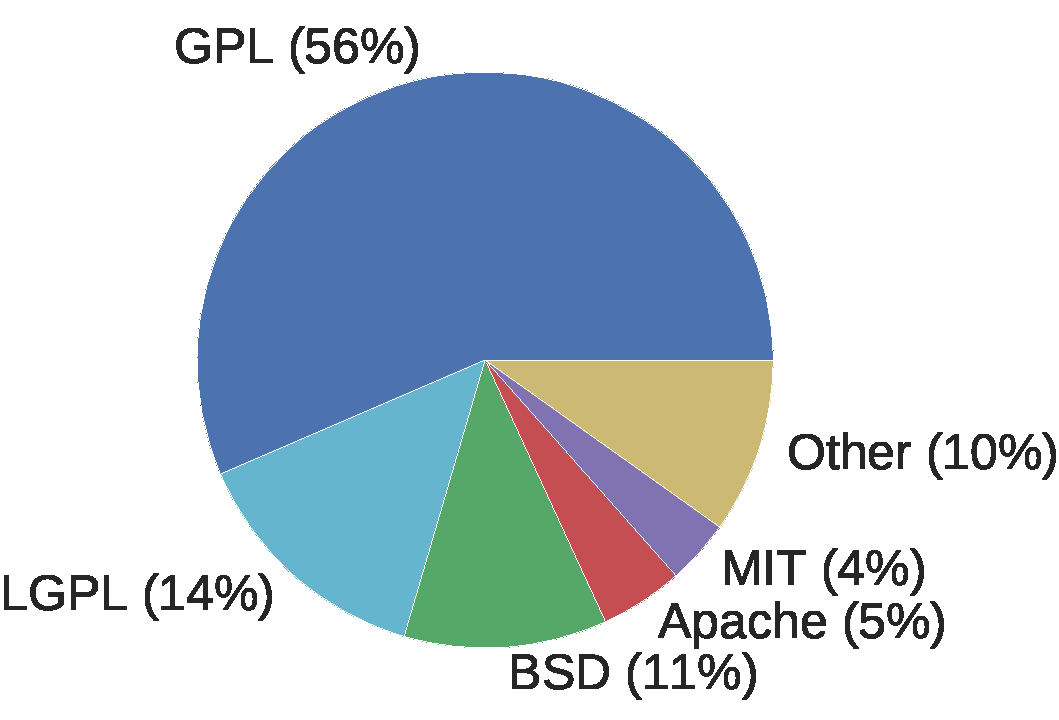
\includegraphics[width=.5\linewidth]{../licenses}
\caption{\label{licenses} Distribution of open-source licenses used in cataloged software packages.}
\end{figure}

\begin{figure*}
\centering
\begin{subfigure}[t]{.4\linewidth}
\centering \label{develop}
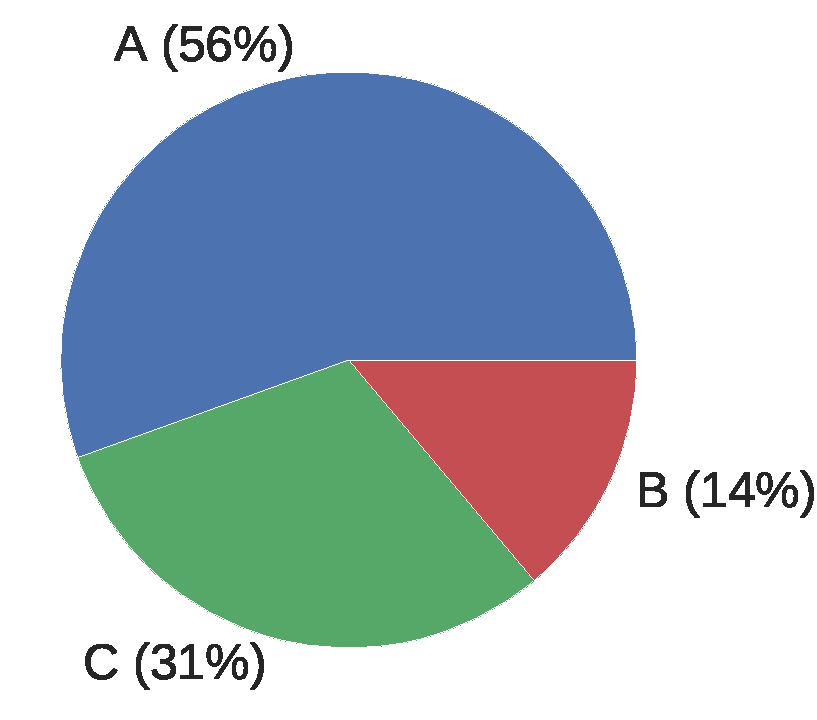
\includegraphics[width=\linewidth]{../develop}
\end{subfigure}
\hfill
\begin{subfigure}[t]{.4\linewidth}
\centering \label{usage}
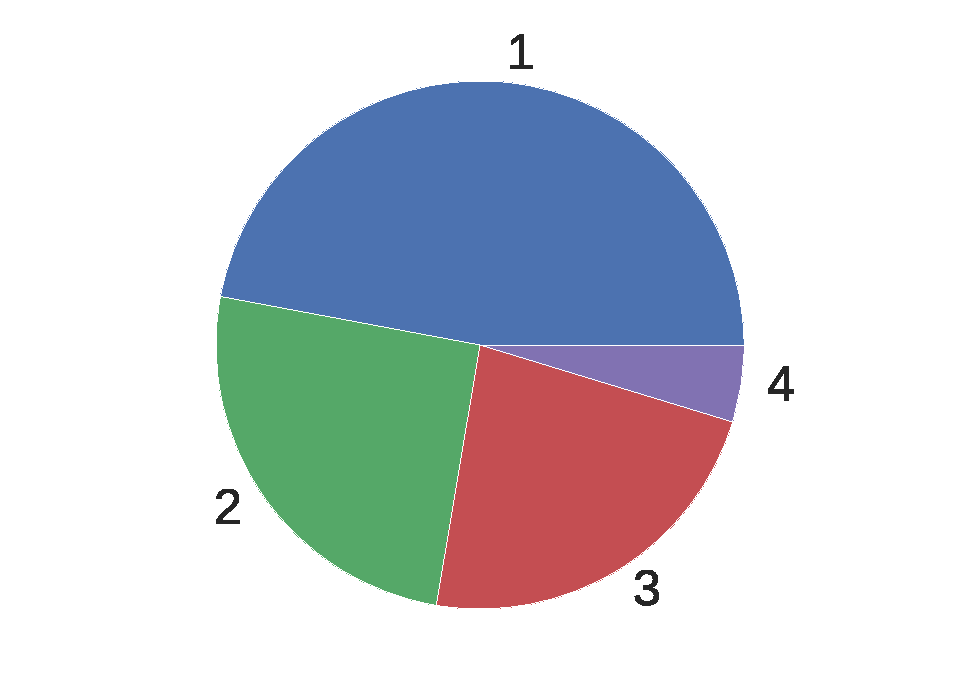
\includegraphics[width=\linewidth]{../usage}
\end{subfigure}
\caption{\label{pies} Activity distributions of cataloged software packages.
\subref{develop} Distribution of development activity. \subref{usage} Distribution of user activity.
}
\end{figure*}

We have cataloged \textbf{X} open-source packages for molecular modeling that provide a wide range of capabilities.  As shown in Figure~\ref{licenses}, the most popular license (\textbf{X\%}) is some variant of the copyleft GNU Public License, which ensures that derivative works remain open-source.  Interestingly \textbf{X\%} of the packages catalog have a corresponding, citeable publication which suggests that much of the software originates from academia.   

A substantial portion of the packages cataloged are under active development and see significant usages, as shown in Figure~\ref{pies}.  We rated \textbf{X\%} of the packages as `A' level development, meaning major features or releases were made within the last 18 months, and \textbf{X\%} see substantial usage (rank 1).  Interestingly, a number of packages (\textbf{X}), despite having received no development for the past 18 months still see significant usage.  